

\documentclass[aos]{imsart} % annals of applied statistics 
\setattribute{journal}{name}{} 

\RequirePackage[OT1]{fontenc}
\RequirePackage{amsthm,amsmath,amssymb}
\RequirePackage[square,authoryear,sort]{natbib}
\RequirePackage[authoryear]{natbib}
\RequirePackage[colorlinks,citecolor=blue,urlcolor=blue]{hyperref}

% settings
%\pubyear{2014}
%\volume{0}
%\issue{0}
%\firstpage{1}
%\lastpage{8}
%\arxiv{arXiv:0000.0000}

\usepackage{macros}
\usepackage{fullpage}
\usepackage[mathcal, mathscr]{eucal}
\usepackage{colortbl}
\usepackage[size=small]{caption}
\usepackage{subcaption}
\usepackage{graphicx}
\graphicspath{{./figures/eps/}}
\DeclareGraphicsExtensions{.pdf,.png,.jpg,.eps}
\usepackage{algorithm}
\usepackage{algorithmic}
\usepackage[authoryear,sort]{natbib}
\setcitestyle{authoryear,square}


\bibpunct[; ]{(}{)}{;}{a}{,}{;} 


\usepackage{booktabs}

\newcommand{\vect}{\boldsymbol}
\newcommand{\matr}{\boldsymbol}
\newcommand{\diag}{\textrm{diag}}

\newcommand{\specialcell}[2][c]{%
  \begin{tabular}[#1]{@{}c@{}}#2\end{tabular}}
  
\endlocaldefs

\begin{document}

\begin{frontmatter}
\title{Fully Bayesian inference of interpretable structure underlying neural spike trains} 
\runtitle{Inference of interpretable structure in neural spike trains}
\begin{aug}
\author{\fnms{Scott W.} \snm{Linderman},\thanksref{t1}\ead[label=e1]{swl@seas.harvard.edu}}
\author{\fnms{Ryan P.} \snm{Adams},\thanksref{t2}\ead[label=e2]{rpa@seas.harvard.edu}}
\and
\author{\fnms{Jonathan W.} \snm{Pillow} \thanksref{t3}\ead[label=e3]{pillow@princeton.edu}}

\thankstext{t1}{Supported by the Center for Brains, Minds and Machines (CBMM), funded by NSF STC award CCF-1231216. }
\thankstext{t2}{}
\thankstext{t3}{}

\runauthor{S. W. Linderman, R. P. Adams, and J. W. Pillow}

\affiliation{Harvard University, Harvard University, Princeton University} 
\address{Scott W. Linderman\\
School of Engineering and Applied Science \\
Harvard University\\
Cambridge, MA 02138,  USA\\
\printead{e1}
}

\address{Ryan P. Adams\\
School of Engineering and Applied Science \\
Harvard University\\
Cambridge, MA 02138,  USA\\
\printead{e2}
}

\address{Jonathan Pillow\\
Princeton Neuroscience Institute \\
Princeton University\\
Princeton, NJ 08544, USA\\
\printead{e3}
}

\end{aug}

\begin{abstract} 
With the steady expansion of neural recording capability comes the promise that unexpected patterns will be found and novel insights will be gleaned about neural computation.  Toward realizing this goal, we present a negative binomial spike train model parameterized by a network of functional interactions between neurons. Under this network we introduce prior distributions characterized by interpretable latent variables associated with each neuron, for example a latent class or location.  We leverage recent innovations in negative binomial regression to perform efficient fully-Bayesian inference, and show how the underlying network variables can be inferred alongside the low-dimensional latent variables of each neuron.
\end{abstract}


%\begin{keyword}
%\end{keyword}

%\kwd{}
%\end{keyword}

\end{frontmatter}

\section{Introduction}

\section{Model}
We begin with a matrix of observed spike counts,~$\bS\in\naturals^{T\times N}$, where~$T$ is the number of time bins and~$N$ is the number of recorded neurons. Typically, the bin size is taken to be small enough that a only small number of spikes may be observed, for example~10ms. We will model these spike counts as random draws from a negative binomial distribution,
\begin{align}
s_{t,n} &\sim \text{NB}(\xi, p_{t,n}) = {{s_{t,n}+\xi-1}\choose{s_{t,n}}} (1-p_{t,n})^\xi p_{t,n}^{s_{t,n}},
\end{align}
for~$\xi>0$ and~${p_{t,n}\in(0,1)}$. Letting~${\lambda_{t,n}=\frac{p_{t,n}}{1-p_{t,n}}}$, we have that~$\mathbb{E}[s_{t,n}]=\xi\lambda_{t,n}$ and~${\text{Var}[s_{t,n}] = \xi\lambda_{t,n}(1+\lambda_{t_n})}$. Unlike the Poisson distribution, here the variance can exceed the mean and model overdispersed spike counts. We may arrive at the negative binomial distribution by marginalizing out the firing rate,~$f$, of the Poisson distribution in the following generative model,
\begin{align}
f_{t,n} &\sim \text{Gamma}(\xi, \lambda_{t,n}) \\
s_{t,n} &\sim \text{Poisson}(f_{t,n}).
\end{align}

We proceed by modeling~$\lambda_{t,n}$ with a log linear model. As shown by \citet{Zhou2012} and previously leveraged by~\citet{Scott2012}, we may then capitalize on a number of nice properties of the negative binomial distribution to perform efficient inference. Let,
\begin{align}
\psi_{t,n} \equiv \log \lambda_{t,n} &= x_{t,n} + \epsilon_{t,n}, \\
x_{t,n} &= b_{n} + \sum_{n'=1}^n \, \sum_{\Delta t=1}^{\Delta t_{\mathsf{max}}} h_{n'\to n}[\Delta t] \cdot s_{t-\Delta t, n'},
\end{align}
where~$b_n\in \reals$ is a constant bias;\;~${h_{n'\to n}(\Delta t):\; (0,\Delta t_{\mathsf{max}})\to \reals}$ is a causal, directed impulse response capturing the effect that spikes on neuron~$n'$ have on the activation of neuron~$n$;\; and~${\epsilon_{t,n}\in\reals}$ is an additive noise term. 

Following \citet{Zhou2012}, we introduce Gaussian priors,
\begin{align}
b_n&\sim\distNormal(\mu_b, \sigma_b^2), \\
\epsilon_{t,n}&\sim\distNormal(0, \sigma_\epsilon^2).
\end{align}
As they have shown, by augmenting our data with a set of Polya-Gamma mixing weights, the likelihood will be rendered conjugate with these Gaussian priors.

\subsection{Modeling the Network}
Traditionally, an impulse response~${h_{n'\to n}(\Delta t)}$ is represented by a weighted set of basis functions with Gaussian or group sparsity inducing priors on the coefficients \citep{Pillow2008}. In order to lend greater interpretability to the model we introduce a directed adjacency matrix~$\bA$ that models the sparsity of the functional network. This \emph{spike-and-slab} model \citep{Mitchell1988} allows us to reason about the sparsity and strength of the functional interactions. We begin by decomposing the directed impulse responses as,
\begin{align}
\label{eqn:glm_ir}
h_{n' \to n}[\Delta t] \equiv A_{n'\to n} \,\cdot\, \bw_{n' \to n}^T \br[\Delta t].
\end{align}
Here,~${A_{n'\to n}\in\{0,1\}}$ is a binary random variable indicating the presence of a direct interaction from neuron~$n'$ to neuron~$n$,~~${\bw_{n'\to n} \in \reals^B}$ is a vector of weights corresponding to the~$B$ basis functions~${r_b[\Delta t]}$.  The basis functions are specified a priori. Typical choices of basis functions include exponentially decaying functions and rectified cosine functions \citep{Pillow2008}.


\subsection{Interpretable Latent Network Structure}
% Figure 1: Random graph examples
\begin{figure}[t]
  \centering
  \begin{subfigure}[b]{.3\textwidth}
    \centering
    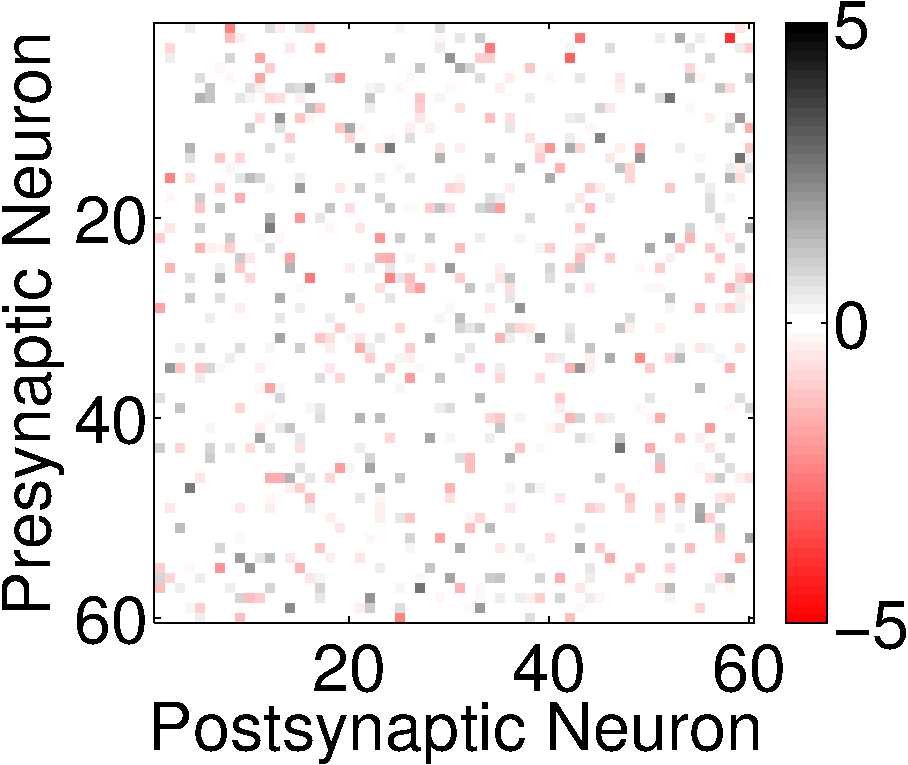
\includegraphics[width=.9\textwidth]{figures/sparse}
    \caption{Erd\H{o}s-Renyi}
    \label{fig:er}
  \end{subfigure}
  \begin{subfigure}[b]{.3\textwidth}
    \centering
    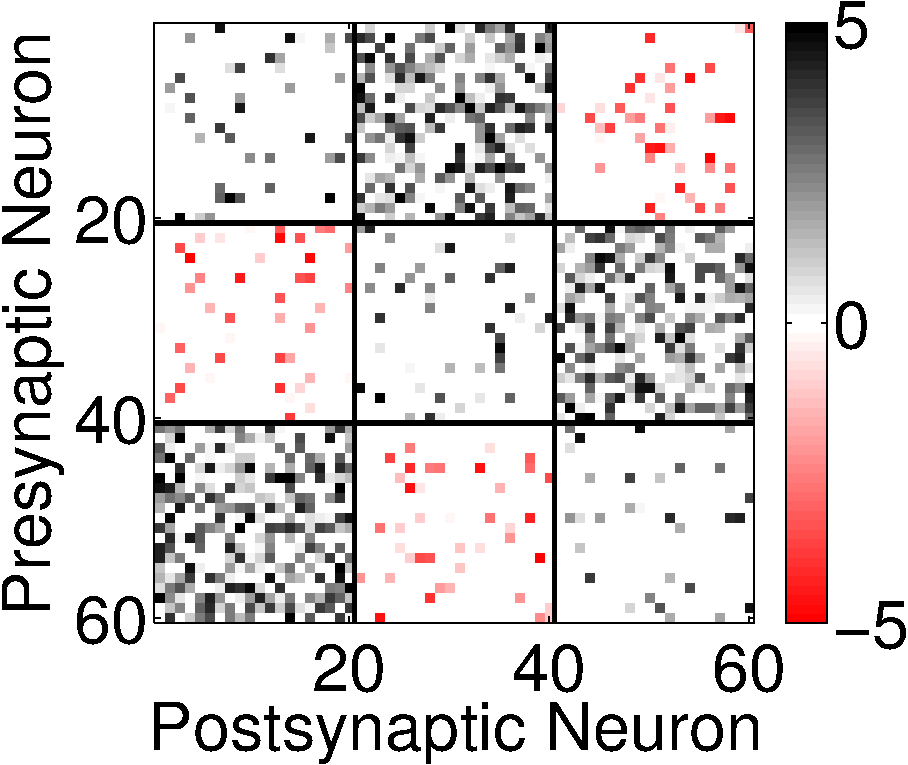
\includegraphics[width=.9\textwidth]{figures/sbm}
    \caption{SBM}
    \label{fig:sbm}
  \end{subfigure}
  \begin{subfigure}[b]{.3\textwidth}
    \centering
    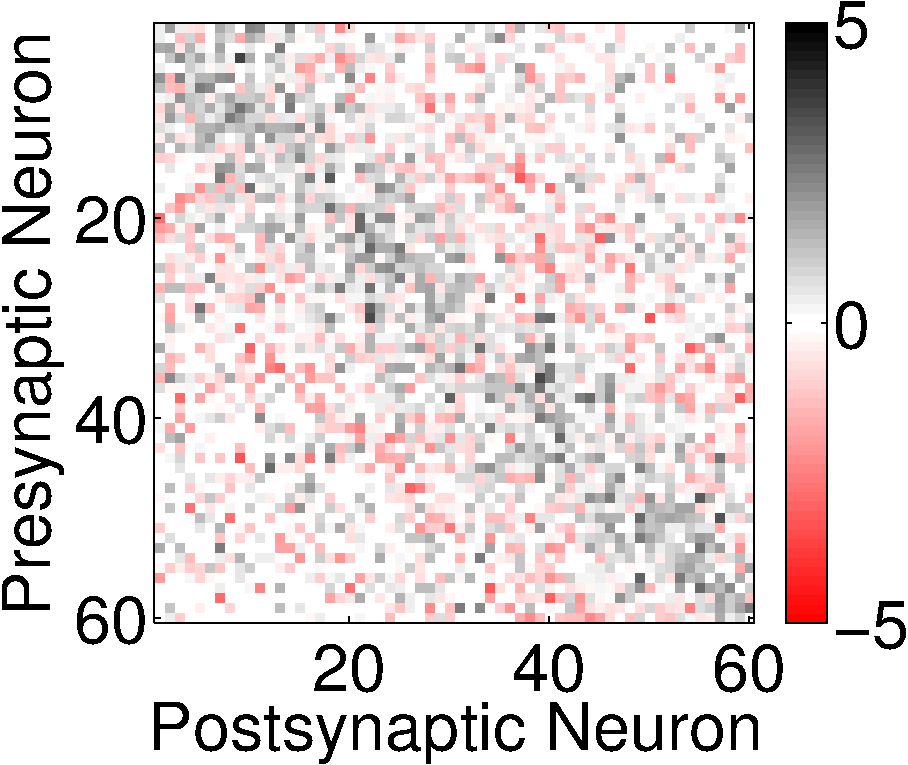
\includegraphics[width=.9\textwidth]{figures/latent_dist}
    \caption{Latent Distance}
    \label{fig:distance}
  \end{subfigure}
  \caption{Examples from a variety of network models. (a) An Erd\H{o}s-Renyi random graph with independent Bernoulli entries in~$\bA$ and Gaussian-distributed weights. (b) A stochastic block model (SBM) with 3 blocks. The block affiliations govern both the weight and the connection probability. (c) A latent distance model in which nearby neurons have dense, excitatory interactions whereas distant neurons have sparse, inhibitory interactions.}
\label{fig:network_models}
\end{figure}

Unfortunately, our reparameterized model still has~$O(N^2)$ parameters.  For large~$N$, this not only exceeds the limits of what we can reasonably interpret, but fitting this model may also require more data than we can handle computationally.

To address this issue, we propose to model the network with latent variables that reflect low dimensional underlying structure. During inference, we will marginalize out the weights of the individual interactions and deal directly with the sparsity pattern and the low dimensional latent variables. We will consider three types of well known latent network models \citep{Hoff2008, Lloyd2012} in detail: Erd\H{o}s-Renyi graphs, stochastic block models (SBMs), and latent distance models. Figure~\ref{fig:network_models} illustrates examples from these three classes.

\paragraph{Erd\H{o}s-Renyi Networks.}
Erd\H{o}-Renyi networks intuitively capture sparse networks. Each weighted connection is an independent, identically distributed random variable. For example, in our model we would have,
\begin{align}
\label{eq:er_A} A_{n' \to n} &\sim \text{Bernoulli}(\rho), \\
\label{eq:er_W} \bw_{n' \to n} &\sim \distNormal(\bmu_W, \bSigma_W).
\end{align}
In this case, the entire network can be represented by only three parameters. Though this dramatically reduces the complexity of our model, it provides little insight into the patterns of functional interaction. In a fully-Bayesian model we place beta and normal-inverse Wishart priors on the parameters,~${\rho \sim \text{Beta}(a_0, b_0)}$ and~${\bmu_W,\bSigma_W \sim \text{NIW}(\bmu_0, \kappa_0, \bSigma_0, \nu_0)}$. 

\paragraph{Stochastic Block Models (SBM's).} One type of structure we might hope to find in functional networks is latent classes of neurons. For example, consider the following generative model:
\begin{align}
c_n &\sim \text{Categorical}(\bp),\\
A_{n' \to n} &\sim \text{Bernoulli}(\rho_{c_{n'}\to c_n}), \\
\bw_{n' \to n} &\sim \distNormal(\bmu_{c_{n'}\to c_n}, \bSigma_{c_{n'}\to c_n}),
\end{align}
where~${\{c_n\} \in [1,\ldots, C]^N}$ is a set of latent ``class'' assignments that determine the distribution over interactions with other neurons. These latent classes might correspond to excitatory versus inhibitory neurons, or to neurons that perform similar computational roles and hence have similar patterns of interaction. For example, in the retina these classes could distinguish ``ON'' and ``OFF'' cells. Here we place a Dirichlet prior over the class probabilities,~$\bp \sim \text{Dirichlet}(\alpha)$, and conjugate priors on the remaining parameters as above.

\paragraph{Latent Distance Models.} Finally, consider a model in which each neuron has a latent location. This location may correspond to a measured location, such as the location of a neuron on the retina, or an abstract location, such as the center of a neuron's tuning curve in some feature space. In this generative model, the probability and strength of an interaction then depends on the distance between a pair of neurons. Let,
\begin{align}
\ell_n &\sim \distNormal(\mu_L, \Sigma_L),\\
A_{n' \to n} &\sim \text{Bernoulli}(\,f_\rho(||\ell_n - \ell_{n'}||)\,), \\
\bw_{n' \to n} &\sim \distNormal(\,f_{\bmu}(||\ell_n - \ell_{n'}||),\; f_{\bSigma}(||\ell_n - \ell_{n'}||)\,),
\end{align}
where~${\ell_n\in \reals^D}$ is the latent location of the neuron, and~${f_\bullet}$ are functions that map distances into probabilities, means, or variances, as appropriate. For example, we may specify that the probability of an interaction decays exponentially with distance,~${f_\rho(\Delta \ell)=\exp\{-\Delta \ell / \tau\}}$. More generally, we could learn these functions under a generic Gaussian process prior.

\paragraph{Composing Network Models.} The network models described above can easily be composed to capture more complicated structure.  Erd\H{o}s-Renyi networks are already clearly a special case of SBM's., but there may be cases where we would like to set an global sparsity level with an Erd\H{o}s-Renyi model and then learn block structure on top of that by letting~${\rho_{n'\to n}=\rho_{ER} \cdot \rho_{c_{n'}\to c_{n}}}$.  This multiplicative combination implements a logical ``AND;'' a logical ``OR'' could be implemented with a softmax function. 

We could also combine SBM's and latent distance models by, for example, we could place a latent distance model on~$\bA$ and a SBM on~$\bW$ by endowing neurons with both a latent class and a latent location. This is a natural model for retinal ganglion cells in which neurons have latent types that determine the sign of their interaction weights, but the probability of an interaction is largely determined by how far apart the two cells are. 

\section{Bayesian Inference}
\citet{Zhou2012} have shown how the negative binomial distribution can be seen as a Polya-Gamma mixture of normals, thereby enable efficient Bayesian inference by data augmentation. The fundamental  property they exploit is that the likelihood as a function of~${\psi_{t,n}=\log \lambda_{t,n}}$ can be written as,
\begin{align}
p(s_{t,n} \given \psi_{t,n}, \xi) &\propto \frac{(e^{\psi_{t,n}})^{s_{t,n}}}{(1 + e^{\psi_{t,n}})^{s_{t,n} + \xi}} \\
& \propto  \exp \left(\frac{s_{t,n}-\xi}{2} \psi_{t,n}\right) \mathbb{E}_{\omega_{t,n}}\left[ \exp\left(-\omega_{t,n} \psi_{t,n}^2 / 2\right)\right],
\end{align}
where~${\omega_{t,n} \sim \text{PG} (s_{t,n}+\xi, 0)}$ and PG denotes the Polya-Gamma distribution. Hence, if we augment our data with Polya-Gamma random variables~${\omega_{t,n}}$, then conditioned on these variables the log likelihood is a quadratic function of~$\psi_{t,n}$ and conjugate with a Gaussian prior.  Specifically, we have,
\begin{align}
\bpsi_n \given \bs_n, \boldsymbol{\omega}_n, \bx_n, \sigma_\epsilon^2 &\sim \distNormal \left( \bbm_{\bpsi}, \bC_{\bpsi}  \right), \\
~
\nonumber \bbm_{\bpsi} &= \bC_{\bpsi} \left[ \frac{\bs_n - \xi}{2}  + \frac{1}{\sigma_{\epsilon}^2} \bx_n \right], \\
~
\nonumber \bC_{\bpsi} &= \left(\frac{1}{\sigma_{\epsilon}^2}\bI + \text{diag}(\boldsymbol{\omega}_n)\right)^{-1}.
\end{align}
Notice that the conditional covariance matrix,~$\bC_{\bpsi}$, is diagonal, and hence the individual time points are uncorrelated. Thus, we do not need to invert the entire matrix and incur an~$O(T^3)$ cost. Rather, each entry can be sampled in parallel given the appropriate computational hardware.

Similarly, the posterior distribution over~$\omega_{t,n}$ can be shown to be Polya-Gamma distributed as well. Gibbs sampling from the posterior distribution then begins as follows:
\begin{align}
\omega_{t,n} &\sim \text{PG}(s_{t,n} + \xi, \psi_{t,n}).
\end{align}
Again, notice that these updates are independent of one another, and hence could be sampled in parallel. The negative binomial parameter~$\xi$ may also be sampled as in \citep{Zhou2012}.

\subsection{Gibbs Sampling the Latent Network Parameters}
Recall that,
\begin{align}
x_{t,n} &= b_{n} + \sum_{n'=1}^n \,A_{n'\to n} \left( \sum_{\Delta t=1}^{\Delta t_{\mathsf{max}}} s_{t-\Delta t, n'} \cdot \br[\Delta t] \bw_{n'\to n} \right) \\
\label{eq:x} &= b_n + \sum_{n'=1}^n \, \bS_{t,n',:} \cdot \hat{\bw}_{n' \to n},
\end{align}
where~${\bS \in \reals^{T \times N \times B}}$ is a tensor of covariates that can be precomputed given the spike train and fixed basis functions with~${\bS_{t,n',:}=\sum_{\Delta t=1}^{\Delta t_{\mathsf{max}}} \br[\Delta t] \cdot s_{t-\Delta t, n'}}$. To simplify notation, we have rewritten our model in terms of the \emph{effective weights},
\begin{align}
\hat{\bw}_{n' \to n} \equiv A_{n' \to n} \cdot \bw_{n' \to n} &\sim \rho \cdot \delta(\hat{\bw}_{n' \to n}) + (1-\rho) \cdot \distNormal(\bmu_{n' \to n}, \bSigma_{n' \to n}).
\end{align}

\paragraph{Joint Gibbs update of~$A_{n' \to n}$ and~$\bw_{n' \to n}$}  We can improve sampling performance in this spike-and-slab model by jointly updating the binary variables~$A_{n' \to n}$ and~$\bw_{n' \to n}$. To do so, we first sample,
\begin{align}
A_{n' \to n} &\sim \int p\left(A_{n' \to n}, \bw_{n' \to n} \given \bpsi, \{\hat{\bw}_{n'' \to n}\}_{n'' \neq n'}, \bmu_{n' \to n}, \bSigma_{n' \to n} \right) \,\mathrm{d}\bw_{n' \to n}.
\end{align}
This integral is trivial when ~$A_{n'\to n}=0$, and, since we are working with a conjugate Gaussian model, we can evaluate this integral in closed form for~$A_{n' \to n}=1$. Given on~$A_{n' \to n}$, the conditional distribution of~$\bw_{n' \to n}$ is Gaussian.

The effective weights for each incoming connection to neuron~$n$ must be sampled serially. We can, however, parallelize the updates for each receiving neuron. That is, the effective weights~$\{\hat{\bw}_{n' \to n}\}_{n'=1}^N$ are conditionally independent of the effective weights~$\{\hat{\bw}_{n' \to n''}\}_{n'=1}^N$. 

\paragraph{Gibbs updates of~$\bmu_{n' \to n}$ and~$\bSigma_{n' \to n}$} 
Given a sample of the effective weights, the means and covariances in Erd\H{o}s-Renyi and SBM networks are conjugate with a normal-inverse Wishart (NIW) prior. For latent distance models the conjugacy will depend upon the relation between means, covariances, and latent distances.

\section{Collapsing Gibbs Sampling of the Latent Network Parameters}
{\textcolor{red} {This is a work in progress. The gist is that we can integrate out the weights and sample the binary indicators given~$\bpsi$,~$\bmu$, and~$\bSigma$, but the conditional distributions are complicated because all of the time points become correlated and the posterior distribution of~$\bSigma$ doesn't have a nice form. In short, instantiating~$\bw$ makes conditional updates easier. }}
\\
Conditioning on the presence or absence of an interaction, we may replace the spike-and-slab prior with a degenerate Gaussian distribution,
\begin{align}
\hat{\bw}_{n' \to n} \given A_{n' \to n}, \bmu_{n' \to n}, \bSigma_{n' \to n} \sim \distNormal \left(A_{n' \to n} \cdot \bmu_{n' \to n},\;A_{n' \to n} \cdot \bSigma_{n' \to n} \,\right).
\end{align}
Effectively, when~${A_{n'\to n}}$ equals zero the conditional distribution of the effective weights reduces to a zero-mean, zero-covariance Gaussian.  Concatenating the weight vectors into~${\hat{\bw} = \left[\hat{\bw}_{1 \to n}^\trans, \ldots, \hat{\bw}_{N \to n}^\trans\right]^\trans \in \reals^{NB}}$, we have,
\begin{align}
p\left(\hat{\bw} \given \{A_{n'\to n}, \bu_{n' \to n}, \bSigma_{n' \to n}\}_{n'=1}^N \right) &= \distNormal(\bGamma\bmu, \; \bGamma\bSigma\bGamma^\trans) 
\end{align}
where
\begin{align}
\bmu = \begin{bmatrix} \hat{\bmu}_{1 \to n} \\ \vdots \\ \hat{\bmu}_{N \to n} \end{bmatrix},\;  
\bSigma &= 
	\begin{bmatrix} \bSigma_{1 \to n} &         & \boldsymbol{0} \\
		                              & \ddots  &        \\
		            \boldsymbol{0}    &         & \bSigma_{N \to n} 
	\end{bmatrix}, 
\;
\bGamma = 
	\begin{bmatrix} A_{1 \to n} \bI_B &         & \boldsymbol{0} \\
		                              & \ddots  &        \\
		            \boldsymbol{0}    &         & A_{N \to n} \bI_B 
	\end{bmatrix}
\end{align}


Since Equation~\ref{eq:x} now reduces to a linear function of Gaussians, we can rewrite the prior distribution of~${\bpsi_n\equiv [\psi_{1,n},\ldots,\psi_{T,n}]^\trans \in \reals^T}$ as a multivariate Gaussian,
\begin{align}
p(\bpsi_n \given \hat{\bs}, \bA, \bmu, \bSigma, \mu_b, \sigma_b^2) &= \distNormal(\bmu_{\bpsi}, \bSigma_{\bpsi}) \\
~
\bmu_{\bpsi} &= \mu_b \bone_T + \hat{\bS} \bGamma \bmu \\
~
\bSigma_{\bpsi} &= \sigma_b^2\bone\bone^\trans + \hat{\bS} \bGamma \bSigma \bGamma^T \hat{\bS}^\trans + \sigma_\epsilon^2 \bI_T  \\
~
\hat{\bS} &= \left[\hat{\bs}_1, \ldots, \hat{\bs}_N\right] \in \reals^{T\times NB}, 
\end{align}

Now, having collapsed out the weights~$\bw_{n' \to n}$, we are left with the following conditional distributions:
\begin{align}
p(\bpsi_n \given \bs_n, \boldsymbol{\omega}_n, \xi, \hat{\bS}, \bA, \bmu, \bSigma, \mu_b, \sigma_b^2) &= \distNormal\left(\bpsi \given \bbm_{\bpsi}, bC_{\bpsi}\right),
\end{align}
where~${\boldsymbol{\Omega} = \text{diag}(\boldsymbol{\omega_n})}$ and
\begin{align}
\bbm_{\bpsi} &= \bC_{\bpsi}  \left( \bSigma_{\bpsi}^{-1} \bmu_{\bpsi} + \left( \frac{\bs_n - \xi}{2} \right) \right) \\
~
\bC_{\bpsi} &= \left(\bSigma_{\bpsi}^{-1} + \bOmega\right)^{-1}
\end{align}
Unfortunately this is difficult to sample since~$\bC_{\bpsi}$ is not diagonal. At first glance, it seems that this will require an~$O(T^3)$ cost to factorize the covariance matrix. However, it also seems promising that we could leverage the fact that the covariance matrix is diagonal plus low rank to sample more efficiently. \TODO{Work out the details.}

\paragraph{Sampling~$\bmu$,~$\bSigma$,~$\sigma_b^2$, and~$\sigma_\epsilon^2$ } Given~$\bpsi$ and~$\bGamma$, the likelihood as a function of~$\bmu$ is conjugate with a Gaussian prior. Sampling~$\bmu$ is effectively like sampling the coefficients in a Bayesian linear regression. \TODO{Work out the details.}

Gibbs sampling~$\bSigma$ seems more challenging since~$\bSigma_{\bpsi}$ is a quadratic function of~$\bSigma$. We'll consider the case where~$\bSigma=\sigma_w^2\bI$. Then,
\begin{align}
p(\bpsi_n \given \hat{\bs}, \bA, \bmu, \bSigma, \mu_b, \sigma_b^2) &= \distNormal(\bmu_{\bpsi}, \; \sigma_b^2\bone\bone^\trans + \sigma_w^2 \hat{\bS} \bGamma \bGamma^\trans \hat{\bS}^\trans + \sigma_\epsilon^2 \bI_T).
\end{align}
This does not have a simple conjugate prior for~$\sigma_w$, but we can use an inverse gamma prior and slice sample this parameter. We use the same approach to sample~$\sigma_b^2$ and~$\sigma_\epsilon^2$.

\section{Results}

\section{Conclusion}

\bibliographystyle{imsart-nameyear}
{\small \bibliography{draft}}

\appendix
\section{Logistic Poisson model}
Will the Poisson GLM with a logistic link function yield a similar inference algorithm? We have the following likelihood,
\begin{align}
\label{eq:poisson_lkhd}
p(s_{n,t} \given \lambda_{n}^{\mathsf{max}}, x_{n,t}) &= \frac{1}{s_{n,t}!} \left(\lambda_{n}^{\mathsf{max}} \sigma(x_{n,t}) \right)^{s_{n,t}}  \exp\left\{-\lambda_{n}^{\mathsf{max}} \sigma(x_{n,t}) \right\}.
\end{align}
To use the Polya-gamma augmentation, we want this in the form of~$(e^x)^a / (1 + e^x)^b$. We can make an approximation to Equation~\ref{eq:poisson_lkhd} by using the identity,~${e^x = \lim_{m\to \infty} (1+x/m)^m}$ and substituting~$m=\lambda_n^{\mathsf{max}}$. This yields,
\begin{align}
p(s_{n,t} \given \lambda_{n}^{\mathsf{max}}, x_{n,t}) &\approx \frac{1}{s_{n,t}!} \left(\lambda_{n}^{\mathsf{max}} \sigma(x_{n,t}) \right)^{s_{n,t}}  \left(1-\frac{\lambda_{n}^{\mathsf{max}} \sigma(x_{n,t})}{\lambda_{n}^{\mathsf{max}}} \right)^{\lambda_{n}^{\mathsf{max}}}, \\
&= \frac{1}{s_{n,t}!} \left(\lambda_{n}^{\mathsf{max}} \sigma(x_{n,t}) \right)^{s_{n,t}}  \left(1-\sigma(x_{n,t}) \right)^{\lambda_{n}^{\mathsf{max}}}, 
\\
&= \frac{1}{s_{n,t}!} \left(\lambda_{n}^{\mathsf{max}}\right)^{s_{n,t}} \left(\frac{e^{x_{n,t}}}{1+e^{x_{n,t}}} \right)^{s_{n,t}}  \left(\frac{1}{1+e^{x_{n,t}}} \right)^{\lambda_{n}^{\mathsf{max}}}, \\ 
&= \frac{1}{s_{n,t}!} \left(\lambda_{n}^{\mathsf{max}}\right)^{s_{n,t}} \frac{\left(e^{x_{n,t}}\right)^{s_{n,t}}}{\left(1+e^{x_{n,t}} \right)^{s_{n,t} + \lambda_{n}^{\mathsf{max}}}}.
\end{align}

This is essentially reversing the standard derivation of the Poisson as a limiting case of the Binomial distribution for large number of trials (in this case, large~$\lambda_n^{\mathsf{max}}$).  \emph{We might be able to make this more precise by lower bounding the likelihood with this more manageable expression. Then we could rejection sample by drawing ~$u\sim\text{Unif}(0,e^x)$  and using the Polya-gamma trick when~$u\leq(1-x/m)^m$, and falling back to a slower form of sampling when~$(1-x/m)^m < u \leq e^x$.}

Given~$s_{n,t}$ and~$\lambda_n^{\mathsf{max}}$, the likelihood of~$x_{n,t}$ has the necessary form for the Polya-gamma augmentation. Given~$s_{n,t}$ and~$x_{n,t}$, the likelihood of~$\lambda_n^{\mathsf{max}}$ is conjugate with a gamma prior.



\end{document}

   
